\documentclass[12pt]{article}
\usepackage{CJK}
\usepackage{graphicx}
\usepackage{subfigure}
\usepackage{amsfonts,amssymb,amsmath}

%\begin{CJK*}{UTF8}{song}
\begin{document}
\title{Toy Data and Experiment Settings}
%\institute{09300240004}
%\frame{\titlepage}

\maketitle
\section{Toy Data}
Documents in the real world are mixtures of topic-specific words like proper names, and also frequent words like articles, pronouns and conjunctions. In other situations where documents and words a artificially and conceptually defined, as in our situation where each day corresponds to two words describing raise or fall in stock price, noises are also inevitable. Toy data is introduced in order to test the robustness of our model against noise words. And also, for the reason to illustrate the performance of our model in cases where two views are well-related, partially related, or unrelated, the toy data should be able to generate different $A$'s.

There are three parameters to determine topic-word distributions, $p_u$, $W_n$, $W_t$, and $n_t$. Each of the $n_t$ topics in the current view has $W_t$ topic-specific words, each of which has a probability of $1/(p_un_tW_n+n_tW_t)$. For the $W_n$ noise words, their probability is constant through all topics, and is $p_u$-times of the topic-specific words. The following matrix $P$ shows an example where $p_u=0.1, W_n=4, n_t=3, W_t=2$:

\begin{equation*}
\left(          
  \begin{array}{cccccccccc}   
    0.138 & 0.138 & 0& 0& 0& 0& 0.013 & 0.013 & 0.013 & 0.013 \\
    0& 0& 0.138 & 0.138 & 0& 0& 0.013 & 0.013 & 0.013 & 0.013 \\
    0& 0& 0& 0& 0.138 & 0.138 & 0.013 & 0.013 & 0.013 & 0.013 \\
  \end{array}
\right)^\top
\end{equation*}

The interdependency between two views can be measured by considering $A$ as the joint distribution of two (latent topic) random variables, $W$ and $Z$. Thus, its mutual information entropy represented the expected value of information we can get about $Z$ from $W$, or vice versa. However, we cannot operate the entropy directly. Noticed that when the joint distribution is uniform, or some (i, j) has probability of 1, the entropy reaches its minimum, and this hints us that by controlling the variance of $A$ we can have different entropy.

For the reason that our toy data has no physical meaning, the elements in matrix $A$ may get exchanged without impacting $P$ and $Q$, and we can take them lining up to a $st$-dimensional vector. Though a $st$-dimensional Gamma distribution is preferred to ensure the sum to be 1, here we adopt $st$ times of sampling a Beta distribution $B(\alpha, \beta)$ and check the sum instead, to cut short time expense. Parameters $(\alpha, \beta)$ is given by the following equations \ref{eqn_alpha_beta_choosing_start} to \ref{eqn_alpha_beta_choosing_end}, and $c$ is the only parameter needed to generate different $A$'s. Beta distribution is a good choice for its PDF gets non-zeros only in $[0, 1]$. In practice, the parameter $c$ is changing in $[0, 0.9]$.

\begin{eqnarray}
\label{eqn_alpha_beta_choosing_start}
\eta = \frac{1}{\mu} - 1 = st - 1 \\
\sigma = c \sigma_m \\
\alpha = \frac{\frac{\eta}{\sigma^2(1+\eta^2)}-1}{1+\eta} \\
\beta = \eta \alpha \\
\sigma_m = \sqrt{\frac{1}{st} \left( \frac{st-1}{(st)^2} + \left( \frac{1}{st} - 1 \right)^2 \right)} \approx \sqrt{1/st}
\label{eqn_alpha_beta_choosing_end}
\end{eqnarray}

\begin{figure}
\small
\centering
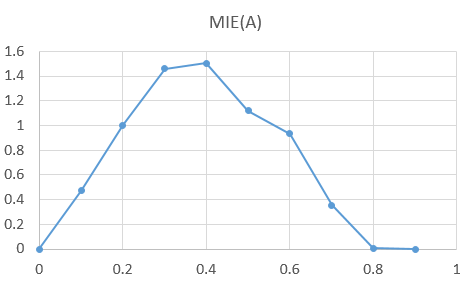
\includegraphics[width=0.5\textwidth]{c_vs_ent.png}
\caption{$c$ versus mutual information entropy of generated $A$'s}
\label{fig_c_vs_ent}
\end{figure}

\section{Stock data}
We built a selected collection of stock price data and their BSDs to examine the performance of our model in practical scenes. This collection is composed of 50 stocks in China's A-share market, from 5 different industries (banking, pharmaceutical, IT, steel and wine).

To represent the BSD data, we simply use its word-frequency data, and all stop-words and punctuations are reserved since we need them to examine the robustness of our model against noise words. 

%To represent the price data, the daily percentage of price spread is involved, and we correspond two dimensions to each day, one for up and one for down, in order to eliminate negative values. The price data, too, is handled as word-frequency.

%上面这段也可以说
We build a $2T$-dimensional vector $v$ to represent the price data of one stock in a given range of time $0$ ~ $T$ by assigning each $v_i (i=1,2,...,2T)$ to the percentage of price rise on day $(i+1)/2$ if $i$ is odd and that of price fall on day $i/2$ if $i$ is even. We chose two time periods for price data: one is from May 4, 2012 to Sep 27, 2012, and the other dates from Sep 27, 2012 to Dec 31, 2012.

\section{Experiment Settings}
Since the initial values will vary the result of our model, different measures of initialization is examined in our experiments. We examine LDA, PLSA, K-means (denoted as `kmeans'), K-means with Random Projection (`rp'), NNMF (`nn') and NNMF3 (`nn3').

When using LDA, PLSA and K-means, we perform them once on each view, and initialize $P$ and $Q$ using their word-topic matrix (LDA, PLSA) or centroids (K-means). We label the objects with a pair of labels from the two clusterings when comparing purity or NMI with the clustering result of our method. Random Projection is used to reduce data dimension, and the clustering is also done by K-means. NNMF is used to factorize data on two views respectively. (i.e., assumed that the data in View 1 is represented by a $p \times N$ matrix $D_1$ and the data in View 2 is $D_2 \in \mathbb{R}^{q \times N}$, the initial $P = \text{normalize}(\text{nnmf}(D_1, s))$ and $Q = \text{normalize}(\text{nnmf}(D_1, t))$, where the function `normalize' normalizes the 1-norm of each row vector to 1.) In NNMF3, we perform NNMF twice on the expectation matrix $E$, so that we get three matrices $A \in \mathbb{R}^{p \times s}, B \in \mathbb{R}^{s \times t}, C \in \mathbb{R}^{t \times q}$ s.t. $E \approx ABC$ wrt. least square error, and the initial $P = normalize(A)$, $Q = normalize(C')$. Noted that in our iterations solving $A$, we also try to increase the mutual information entropy of $A$, so that initial $P$ and $Q$ will also change.

\section{Evaluation}

% 下面这个是照抄 Local Learning Regularized Nonnegative Matrix Factorization 的。

To evaluate the clustering results, we adopt the performance measures used in [Cai et al., 2008]. These performance measures are the standard measures widely used for clustering.

\paragraph{Clustering Accuracy} Clustering Accuracy discovers the one-to-one relationship between clusters and classes and measures the extent to which each cluster contained data points from the corresponding class. Clustering Accuracy is defined as follows:

\begin{equation}
Acc = \frac{\sum_{i=1}^{n}\delta(map(r_i),l_i)}{n}
\end{equation}
where $r_i$ denotes the cluster label of $x_i$, and $l_i$ denotes the true class label, $n$ is the total number of documents, $\delta(x, y)$ is the delta function that equals one if $x = y$ and equals zero otherwise, and $map(r_i)$ is the permutation mapping function that maps each cluster label $r_i$ to the equivalent label from the data set.

\paragraph{Normalized Mutual Information} The second measure is the Normalized Mutual Information (NMI), which is used for determining the quality of clusters. Given a clustering result,
the NMI is estimated by:

\begin{equation}
NMI = \frac{\sum_{k=1}^{C_1}\sum_{m=1}^{C_2}n_{k,m} \log \frac{nn_{k,m}}{n_k\hat{n}_m}}{\sqrt{(\sum_{k=1}^{C_1}n_k \log \frac{n_k}{n})(\sum_{m=1}^{C_2} \hat{n}_m \log \frac{\hat{n}_m}{n})}}
\end{equation}

where $n_k$ denotes the number of data contained in the cluster $D_k(1 \le k \le C_1)$, $n_m$ is the number of data belonging to the $L_m (1 \le m \le C_2)$, and $n_{k,m}$ denotes the number of data that are in the intersection between the cluster $D_k$ and the class $L_m$. The larger the NMI is, the better the clustering result will be.

\end{document}